% Created by tikzDevice version 0.9 on 2016-01-11 22:38:37
% !TEX encoding = UTF-8 Unicode
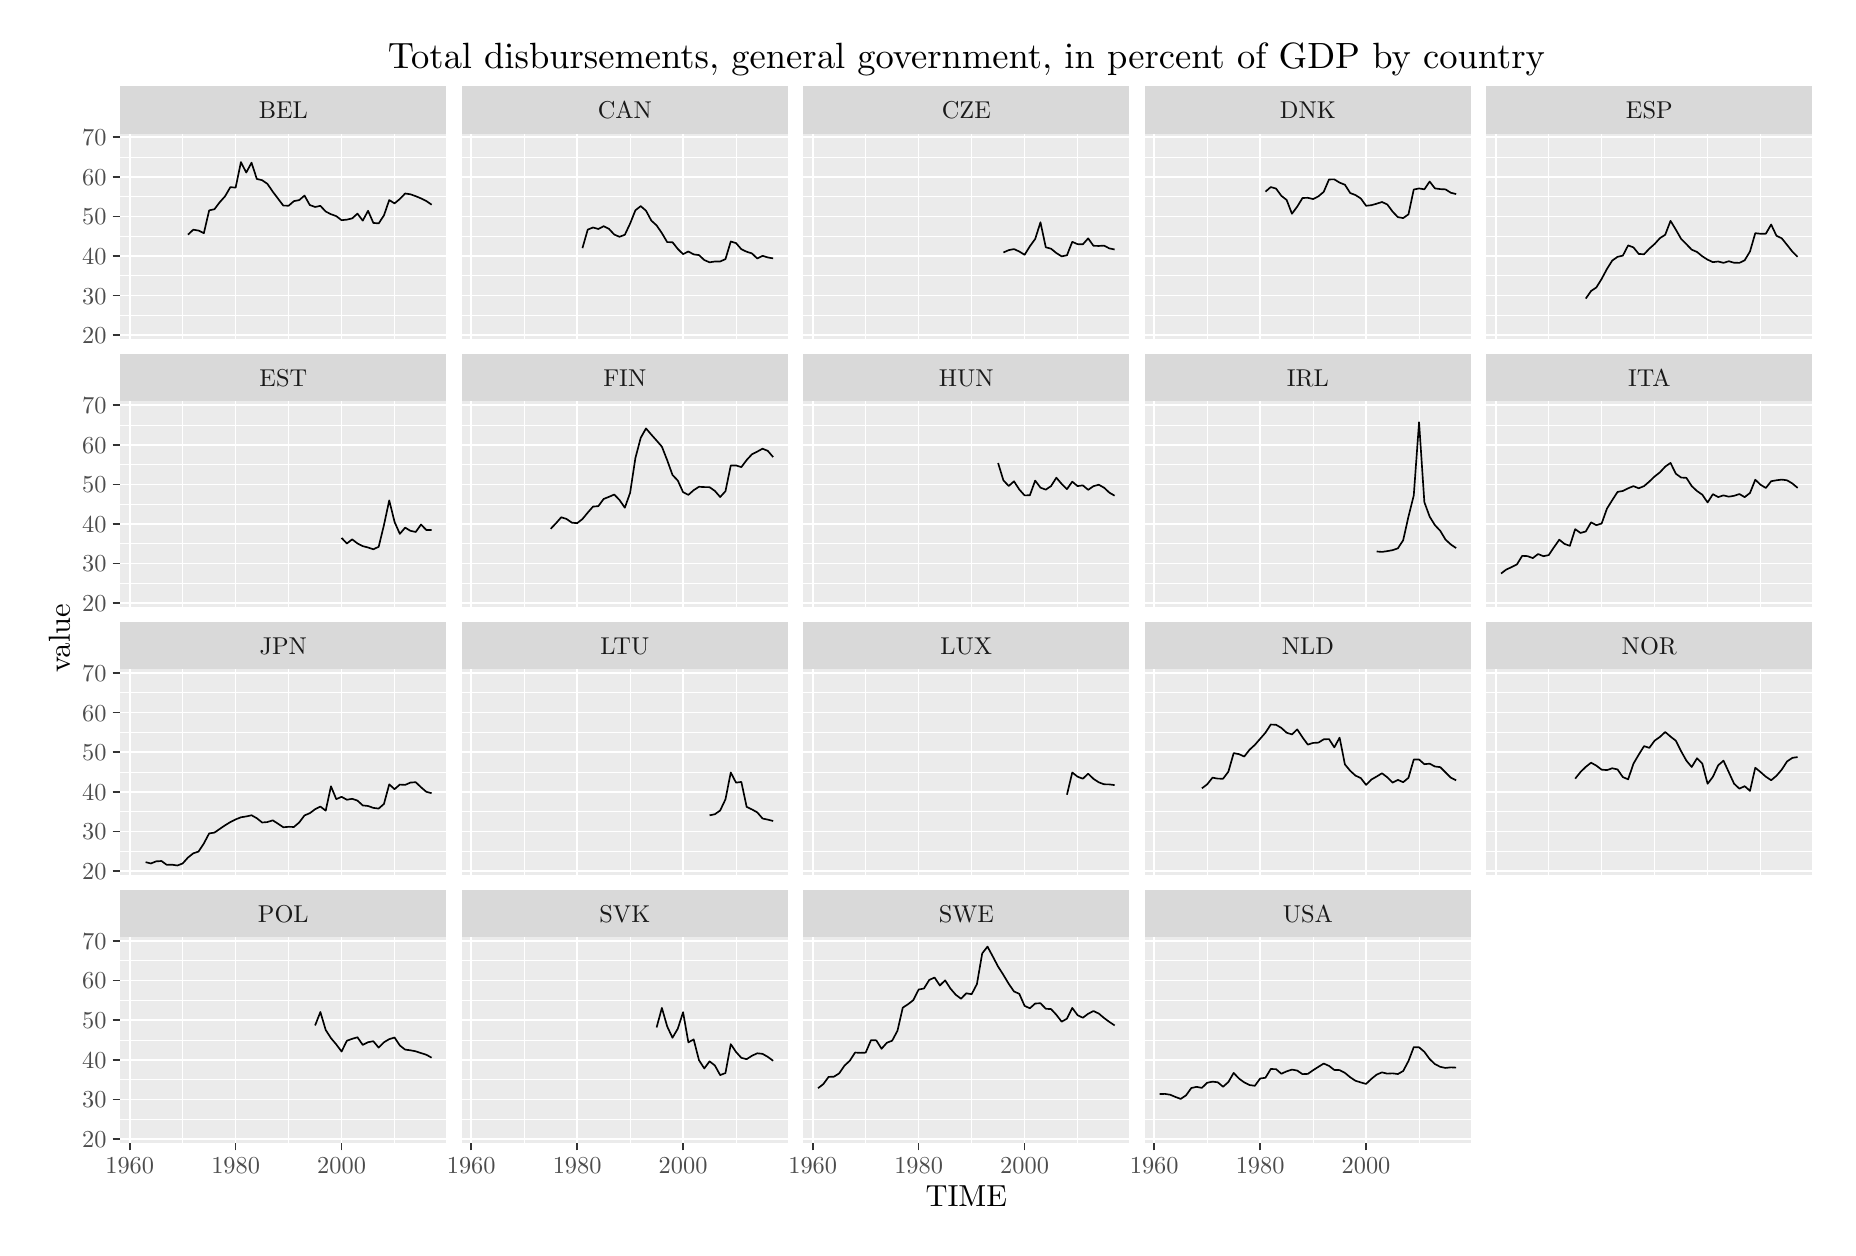
\begin{tikzpicture}[x=1pt,y=1pt]
\definecolor{fillColor}{RGB}{255,255,255}
\path[use as bounding box,fill=fillColor,fill opacity=0.00] (0,0) rectangle (650.43,433.62);
\begin{scope}
\path[clip] (  0.00,  0.00) rectangle (650.43,433.62);
\definecolor{drawColor}{RGB}{255,255,255}
\definecolor{fillColor}{RGB}{255,255,255}

\path[draw=drawColor,line width= 0.6pt,line join=round,line cap=round,fill=fillColor] (  0.00,  0.00) rectangle (650.43,433.62);
\end{scope}
\begin{scope}
\path[clip] ( 33.42,321.12) rectangle (151.33,395.37);
\definecolor{fillColor}{gray}{0.92}

\path[fill=fillColor] ( 33.42,321.12) rectangle (151.33,395.37);
\definecolor{drawColor}{RGB}{255,255,255}

\path[draw=drawColor,line width= 0.3pt,line join=round] ( 33.42,329.62) --
	(151.33,329.62);

\path[draw=drawColor,line width= 0.3pt,line join=round] ( 33.42,343.94) --
	(151.33,343.94);

\path[draw=drawColor,line width= 0.3pt,line join=round] ( 33.42,358.25) --
	(151.33,358.25);

\path[draw=drawColor,line width= 0.3pt,line join=round] ( 33.42,372.57) --
	(151.33,372.57);

\path[draw=drawColor,line width= 0.3pt,line join=round] ( 33.42,386.88) --
	(151.33,386.88);

\path[draw=drawColor,line width= 0.3pt,line join=round] ( 56.01,321.12) --
	( 56.01,395.37);

\path[draw=drawColor,line width= 0.3pt,line join=round] ( 94.29,321.12) --
	( 94.29,395.37);

\path[draw=drawColor,line width= 0.3pt,line join=round] (132.57,321.12) --
	(132.57,395.37);

\path[draw=drawColor,line width= 0.6pt,line join=round] ( 33.42,322.47) --
	(151.33,322.47);

\path[draw=drawColor,line width= 0.6pt,line join=round] ( 33.42,336.78) --
	(151.33,336.78);

\path[draw=drawColor,line width= 0.6pt,line join=round] ( 33.42,351.10) --
	(151.33,351.10);

\path[draw=drawColor,line width= 0.6pt,line join=round] ( 33.42,365.41) --
	(151.33,365.41);

\path[draw=drawColor,line width= 0.6pt,line join=round] ( 33.42,379.73) --
	(151.33,379.73);

\path[draw=drawColor,line width= 0.6pt,line join=round] ( 33.42,394.04) --
	(151.33,394.04);

\path[draw=drawColor,line width= 0.6pt,line join=round] ( 36.87,321.12) --
	( 36.87,395.37);

\path[draw=drawColor,line width= 0.6pt,line join=round] ( 75.15,321.12) --
	( 75.15,395.37);

\path[draw=drawColor,line width= 0.6pt,line join=round] (113.43,321.12) --
	(113.43,395.37);
\definecolor{drawColor}{RGB}{0,0,0}

\path[draw=drawColor,line width= 0.6pt,line join=round] ( 57.92,358.82) --
	( 59.84,360.62) --
	( 61.75,360.30) --
	( 63.66,359.34) --
	( 65.58,367.59) --
	( 67.49,368.02) --
	( 69.41,370.55) --
	( 71.32,372.68) --
	( 73.23,375.97) --
	( 75.15,375.84) --
	( 77.06,385.05) --
	( 78.98,381.26) --
	( 80.89,384.82) --
	( 82.80,378.96) --
	( 84.72,378.49) --
	( 86.63,377.19) --
	( 88.55,374.37) --
	( 90.46,371.85) --
	( 92.37,369.32) --
	( 94.29,369.28) --
	( 96.20,370.93) --
	( 98.12,371.31) --
	(100.03,372.95) --
	(101.94,369.53) --
	(103.86,368.83) --
	(105.77,369.23) --
	(107.69,367.18) --
	(109.60,366.21) --
	(111.51,365.51) --
	(113.43,364.05) --
	(115.34,364.25) --
	(117.26,364.70) --
	(119.17,366.43) --
	(121.08,363.88) --
	(123.00,367.46) --
	(124.91,363.06) --
	(126.83,362.89) --
	(128.74,365.78) --
	(130.65,371.33) --
	(132.57,370.11) --
	(134.48,371.72) --
	(136.40,373.70) --
	(138.31,373.41) --
	(140.22,372.72) --
	(142.14,371.92) --
	(144.05,370.97) --
	(145.97,369.65);
\end{scope}
\begin{scope}
\path[clip] (156.83,321.12) rectangle (274.73,395.37);
\definecolor{fillColor}{gray}{0.92}

\path[fill=fillColor] (156.83,321.12) rectangle (274.73,395.37);
\definecolor{drawColor}{RGB}{255,255,255}

\path[draw=drawColor,line width= 0.3pt,line join=round] (156.83,329.62) --
	(274.73,329.62);

\path[draw=drawColor,line width= 0.3pt,line join=round] (156.83,343.94) --
	(274.73,343.94);

\path[draw=drawColor,line width= 0.3pt,line join=round] (156.83,358.25) --
	(274.73,358.25);

\path[draw=drawColor,line width= 0.3pt,line join=round] (156.83,372.57) --
	(274.73,372.57);

\path[draw=drawColor,line width= 0.3pt,line join=round] (156.83,386.88) --
	(274.73,386.88);

\path[draw=drawColor,line width= 0.3pt,line join=round] (179.41,321.12) --
	(179.41,395.37);

\path[draw=drawColor,line width= 0.3pt,line join=round] (217.69,321.12) --
	(217.69,395.37);

\path[draw=drawColor,line width= 0.3pt,line join=round] (255.97,321.12) --
	(255.97,395.37);

\path[draw=drawColor,line width= 0.6pt,line join=round] (156.83,322.47) --
	(274.73,322.47);

\path[draw=drawColor,line width= 0.6pt,line join=round] (156.83,336.78) --
	(274.73,336.78);

\path[draw=drawColor,line width= 0.6pt,line join=round] (156.83,351.10) --
	(274.73,351.10);

\path[draw=drawColor,line width= 0.6pt,line join=round] (156.83,365.41) --
	(274.73,365.41);

\path[draw=drawColor,line width= 0.6pt,line join=round] (156.83,379.73) --
	(274.73,379.73);

\path[draw=drawColor,line width= 0.6pt,line join=round] (156.83,394.04) --
	(274.73,394.04);

\path[draw=drawColor,line width= 0.6pt,line join=round] (160.27,321.12) --
	(160.27,395.37);

\path[draw=drawColor,line width= 0.6pt,line join=round] (198.55,321.12) --
	(198.55,395.37);

\path[draw=drawColor,line width= 0.6pt,line join=round] (236.83,321.12) --
	(236.83,395.37);
\definecolor{drawColor}{RGB}{0,0,0}

\path[draw=drawColor,line width= 0.6pt,line join=round] (200.46,353.95) --
	(202.38,360.65) --
	(204.29,361.41) --
	(206.21,360.86) --
	(208.12,361.87) --
	(210.03,360.93) --
	(211.95,358.86) --
	(213.86,358.05) --
	(215.78,358.78) --
	(217.69,362.82) --
	(219.60,367.63) --
	(221.52,369.13) --
	(223.43,367.48) --
	(225.35,363.91) --
	(227.26,362.17) --
	(229.17,359.38) --
	(231.09,356.12) --
	(233.00,356.09) --
	(234.92,353.67) --
	(236.83,351.78) --
	(238.74,352.74) --
	(240.66,351.69) --
	(242.57,351.44) --
	(244.49,349.65) --
	(246.40,348.83) --
	(248.31,349.12) --
	(250.23,349.14) --
	(252.14,349.98) --
	(254.06,356.35) --
	(255.97,355.76) --
	(257.88,353.56) --
	(259.80,352.65) --
	(261.71,352.05) --
	(263.63,350.20) --
	(265.54,351.18) --
	(267.45,350.58) --
	(269.37,350.25);
\end{scope}
\begin{scope}
\path[clip] (280.23,321.12) rectangle (398.13,395.37);
\definecolor{fillColor}{gray}{0.92}

\path[fill=fillColor] (280.23,321.12) rectangle (398.13,395.37);
\definecolor{drawColor}{RGB}{255,255,255}

\path[draw=drawColor,line width= 0.3pt,line join=round] (280.23,329.62) --
	(398.13,329.62);

\path[draw=drawColor,line width= 0.3pt,line join=round] (280.23,343.94) --
	(398.13,343.94);

\path[draw=drawColor,line width= 0.3pt,line join=round] (280.23,358.25) --
	(398.13,358.25);

\path[draw=drawColor,line width= 0.3pt,line join=round] (280.23,372.57) --
	(398.13,372.57);

\path[draw=drawColor,line width= 0.3pt,line join=round] (280.23,386.88) --
	(398.13,386.88);

\path[draw=drawColor,line width= 0.3pt,line join=round] (302.81,321.12) --
	(302.81,395.37);

\path[draw=drawColor,line width= 0.3pt,line join=round] (341.09,321.12) --
	(341.09,395.37);

\path[draw=drawColor,line width= 0.3pt,line join=round] (379.37,321.12) --
	(379.37,395.37);

\path[draw=drawColor,line width= 0.6pt,line join=round] (280.23,322.47) --
	(398.13,322.47);

\path[draw=drawColor,line width= 0.6pt,line join=round] (280.23,336.78) --
	(398.13,336.78);

\path[draw=drawColor,line width= 0.6pt,line join=round] (280.23,351.10) --
	(398.13,351.10);

\path[draw=drawColor,line width= 0.6pt,line join=round] (280.23,365.41) --
	(398.13,365.41);

\path[draw=drawColor,line width= 0.6pt,line join=round] (280.23,379.73) --
	(398.13,379.73);

\path[draw=drawColor,line width= 0.6pt,line join=round] (280.23,394.04) --
	(398.13,394.04);

\path[draw=drawColor,line width= 0.6pt,line join=round] (283.67,321.12) --
	(283.67,395.37);

\path[draw=drawColor,line width= 0.6pt,line join=round] (321.95,321.12) --
	(321.95,395.37);

\path[draw=drawColor,line width= 0.6pt,line join=round] (360.23,321.12) --
	(360.23,395.37);
\definecolor{drawColor}{RGB}{0,0,0}

\path[draw=drawColor,line width= 0.6pt,line join=round] (352.57,352.38) --
	(354.49,353.23) --
	(356.40,353.61) --
	(358.32,352.73) --
	(360.23,351.54) --
	(362.14,354.62) --
	(364.06,357.27) --
	(365.97,363.28) --
	(367.89,354.26) --
	(369.80,353.74) --
	(371.71,352.18) --
	(373.63,350.98) --
	(375.54,351.37) --
	(377.46,356.23) --
	(379.37,355.39) --
	(381.28,355.32) --
	(383.20,357.48) --
	(385.11,354.80) --
	(387.03,354.74) --
	(388.94,354.86) --
	(390.85,353.86) --
	(392.77,353.46);
\end{scope}
\begin{scope}
\path[clip] (403.63,321.12) rectangle (521.53,395.37);
\definecolor{fillColor}{gray}{0.92}

\path[fill=fillColor] (403.63,321.12) rectangle (521.53,395.37);
\definecolor{drawColor}{RGB}{255,255,255}

\path[draw=drawColor,line width= 0.3pt,line join=round] (403.63,329.62) --
	(521.53,329.62);

\path[draw=drawColor,line width= 0.3pt,line join=round] (403.63,343.94) --
	(521.53,343.94);

\path[draw=drawColor,line width= 0.3pt,line join=round] (403.63,358.25) --
	(521.53,358.25);

\path[draw=drawColor,line width= 0.3pt,line join=round] (403.63,372.57) --
	(521.53,372.57);

\path[draw=drawColor,line width= 0.3pt,line join=round] (403.63,386.88) --
	(521.53,386.88);

\path[draw=drawColor,line width= 0.3pt,line join=round] (426.21,321.12) --
	(426.21,395.37);

\path[draw=drawColor,line width= 0.3pt,line join=round] (464.49,321.12) --
	(464.49,395.37);

\path[draw=drawColor,line width= 0.3pt,line join=round] (502.77,321.12) --
	(502.77,395.37);

\path[draw=drawColor,line width= 0.6pt,line join=round] (403.63,322.47) --
	(521.53,322.47);

\path[draw=drawColor,line width= 0.6pt,line join=round] (403.63,336.78) --
	(521.53,336.78);

\path[draw=drawColor,line width= 0.6pt,line join=round] (403.63,351.10) --
	(521.53,351.10);

\path[draw=drawColor,line width= 0.6pt,line join=round] (403.63,365.41) --
	(521.53,365.41);

\path[draw=drawColor,line width= 0.6pt,line join=round] (403.63,379.73) --
	(521.53,379.73);

\path[draw=drawColor,line width= 0.6pt,line join=round] (403.63,394.04) --
	(521.53,394.04);

\path[draw=drawColor,line width= 0.6pt,line join=round] (407.07,321.12) --
	(407.07,395.37);

\path[draw=drawColor,line width= 0.6pt,line join=round] (445.35,321.12) --
	(445.35,395.37);

\path[draw=drawColor,line width= 0.6pt,line join=round] (483.63,321.12) --
	(483.63,395.37);
\definecolor{drawColor}{RGB}{0,0,0}

\path[draw=drawColor,line width= 0.6pt,line join=round] (447.27,374.36) --
	(449.18,376.02) --
	(451.09,375.48) --
	(453.01,372.86) --
	(454.92,371.36) --
	(456.84,366.39) --
	(458.75,368.95) --
	(460.66,372.07) --
	(462.58,372.14) --
	(464.49,371.68) --
	(466.41,372.67) --
	(468.32,374.29) --
	(470.23,378.77) --
	(472.15,378.80) --
	(474.06,377.62) --
	(475.98,376.86) --
	(477.89,373.87) --
	(479.80,373.13) --
	(481.72,371.90) --
	(483.63,369.26) --
	(485.55,369.47) --
	(487.46,370.01) --
	(489.37,370.62) --
	(491.29,369.74) --
	(493.20,367.16) --
	(495.12,365.15) --
	(497.03,364.81) --
	(498.94,366.16) --
	(500.86,375.14) --
	(502.77,375.52) --
	(504.69,375.21) --
	(506.60,378.02) --
	(508.51,375.54) --
	(510.43,375.28) --
	(512.34,375.18) --
	(514.26,373.96) --
	(516.17,373.49);
\end{scope}
\begin{scope}
\path[clip] (527.03,321.12) rectangle (644.93,395.37);
\definecolor{fillColor}{gray}{0.92}

\path[fill=fillColor] (527.03,321.12) rectangle (644.93,395.37);
\definecolor{drawColor}{RGB}{255,255,255}

\path[draw=drawColor,line width= 0.3pt,line join=round] (527.03,329.62) --
	(644.93,329.62);

\path[draw=drawColor,line width= 0.3pt,line join=round] (527.03,343.94) --
	(644.93,343.94);

\path[draw=drawColor,line width= 0.3pt,line join=round] (527.03,358.25) --
	(644.93,358.25);

\path[draw=drawColor,line width= 0.3pt,line join=round] (527.03,372.57) --
	(644.93,372.57);

\path[draw=drawColor,line width= 0.3pt,line join=round] (527.03,386.88) --
	(644.93,386.88);

\path[draw=drawColor,line width= 0.3pt,line join=round] (549.61,321.12) --
	(549.61,395.37);

\path[draw=drawColor,line width= 0.3pt,line join=round] (587.89,321.12) --
	(587.89,395.37);

\path[draw=drawColor,line width= 0.3pt,line join=round] (626.17,321.12) --
	(626.17,395.37);

\path[draw=drawColor,line width= 0.6pt,line join=round] (527.03,322.47) --
	(644.93,322.47);

\path[draw=drawColor,line width= 0.6pt,line join=round] (527.03,336.78) --
	(644.93,336.78);

\path[draw=drawColor,line width= 0.6pt,line join=round] (527.03,351.10) --
	(644.93,351.10);

\path[draw=drawColor,line width= 0.6pt,line join=round] (527.03,365.41) --
	(644.93,365.41);

\path[draw=drawColor,line width= 0.6pt,line join=round] (527.03,379.73) --
	(644.93,379.73);

\path[draw=drawColor,line width= 0.6pt,line join=round] (527.03,394.04) --
	(644.93,394.04);

\path[draw=drawColor,line width= 0.6pt,line join=round] (530.47,321.12) --
	(530.47,395.37);

\path[draw=drawColor,line width= 0.6pt,line join=round] (568.75,321.12) --
	(568.75,395.37);

\path[draw=drawColor,line width= 0.6pt,line join=round] (607.03,321.12) --
	(607.03,395.37);
\definecolor{drawColor}{RGB}{0,0,0}

\path[draw=drawColor,line width= 0.6pt,line join=round] (563.01,335.72) --
	(564.93,338.46) --
	(566.84,339.75) --
	(568.75,342.83) --
	(570.67,346.43) --
	(572.58,349.46) --
	(574.50,350.81) --
	(576.41,351.25) --
	(578.32,354.94) --
	(580.24,354.22) --
	(582.15,351.86) --
	(584.07,351.73) --
	(585.98,353.76) --
	(587.89,355.45) --
	(589.81,357.56) --
	(591.72,358.79) --
	(593.64,363.81) --
	(595.55,360.65) --
	(597.46,357.30) --
	(599.38,355.37) --
	(601.29,353.40) --
	(603.21,352.57) --
	(605.12,351.00) --
	(607.03,349.79) --
	(608.95,348.89) --
	(610.86,349.12) --
	(612.78,348.63) --
	(614.69,349.22) --
	(616.60,348.67) --
	(618.52,348.63) --
	(620.43,349.55) --
	(622.35,352.74) --
	(624.26,359.35) --
	(626.17,359.14) --
	(628.09,359.18) --
	(630.00,362.48) --
	(631.91,358.44) --
	(633.83,357.50) --
	(635.74,355.13) --
	(637.66,352.70) --
	(639.57,350.81);
\end{scope}
\begin{scope}
\path[clip] ( 33.42,224.31) rectangle (151.33,298.56);
\definecolor{fillColor}{gray}{0.92}

\path[fill=fillColor] ( 33.42,224.31) rectangle (151.33,298.56);
\definecolor{drawColor}{RGB}{255,255,255}

\path[draw=drawColor,line width= 0.3pt,line join=round] ( 33.42,232.81) --
	(151.33,232.81);

\path[draw=drawColor,line width= 0.3pt,line join=round] ( 33.42,247.13) --
	(151.33,247.13);

\path[draw=drawColor,line width= 0.3pt,line join=round] ( 33.42,261.44) --
	(151.33,261.44);

\path[draw=drawColor,line width= 0.3pt,line join=round] ( 33.42,275.76) --
	(151.33,275.76);

\path[draw=drawColor,line width= 0.3pt,line join=round] ( 33.42,290.07) --
	(151.33,290.07);

\path[draw=drawColor,line width= 0.3pt,line join=round] ( 56.01,224.31) --
	( 56.01,298.56);

\path[draw=drawColor,line width= 0.3pt,line join=round] ( 94.29,224.31) --
	( 94.29,298.56);

\path[draw=drawColor,line width= 0.3pt,line join=round] (132.57,224.31) --
	(132.57,298.56);

\path[draw=drawColor,line width= 0.6pt,line join=round] ( 33.42,225.66) --
	(151.33,225.66);

\path[draw=drawColor,line width= 0.6pt,line join=round] ( 33.42,239.97) --
	(151.33,239.97);

\path[draw=drawColor,line width= 0.6pt,line join=round] ( 33.42,254.29) --
	(151.33,254.29);

\path[draw=drawColor,line width= 0.6pt,line join=round] ( 33.42,268.60) --
	(151.33,268.60);

\path[draw=drawColor,line width= 0.6pt,line join=round] ( 33.42,282.91) --
	(151.33,282.91);

\path[draw=drawColor,line width= 0.6pt,line join=round] ( 33.42,297.23) --
	(151.33,297.23);

\path[draw=drawColor,line width= 0.6pt,line join=round] ( 36.87,224.31) --
	( 36.87,298.56);

\path[draw=drawColor,line width= 0.6pt,line join=round] ( 75.15,224.31) --
	( 75.15,298.56);

\path[draw=drawColor,line width= 0.6pt,line join=round] (113.43,224.31) --
	(113.43,298.56);
\definecolor{drawColor}{RGB}{0,0,0}

\path[draw=drawColor,line width= 0.6pt,line join=round] (113.43,249.24) --
	(115.34,247.23) --
	(117.26,248.71) --
	(119.17,247.25) --
	(121.08,246.27) --
	(123.00,245.78) --
	(124.91,245.14) --
	(126.83,246.03) --
	(128.74,253.88) --
	(130.65,262.80) --
	(132.57,255.03) --
	(134.48,250.70) --
	(136.40,252.96) --
	(138.31,251.80) --
	(140.22,251.39) --
	(142.14,254.08) --
	(144.05,252.10) --
	(145.97,252.08);
\end{scope}
\begin{scope}
\path[clip] (156.83,224.31) rectangle (274.73,298.56);
\definecolor{fillColor}{gray}{0.92}

\path[fill=fillColor] (156.83,224.31) rectangle (274.73,298.56);
\definecolor{drawColor}{RGB}{255,255,255}

\path[draw=drawColor,line width= 0.3pt,line join=round] (156.83,232.81) --
	(274.73,232.81);

\path[draw=drawColor,line width= 0.3pt,line join=round] (156.83,247.13) --
	(274.73,247.13);

\path[draw=drawColor,line width= 0.3pt,line join=round] (156.83,261.44) --
	(274.73,261.44);

\path[draw=drawColor,line width= 0.3pt,line join=round] (156.83,275.76) --
	(274.73,275.76);

\path[draw=drawColor,line width= 0.3pt,line join=round] (156.83,290.07) --
	(274.73,290.07);

\path[draw=drawColor,line width= 0.3pt,line join=round] (179.41,224.31) --
	(179.41,298.56);

\path[draw=drawColor,line width= 0.3pt,line join=round] (217.69,224.31) --
	(217.69,298.56);

\path[draw=drawColor,line width= 0.3pt,line join=round] (255.97,224.31) --
	(255.97,298.56);

\path[draw=drawColor,line width= 0.6pt,line join=round] (156.83,225.66) --
	(274.73,225.66);

\path[draw=drawColor,line width= 0.6pt,line join=round] (156.83,239.97) --
	(274.73,239.97);

\path[draw=drawColor,line width= 0.6pt,line join=round] (156.83,254.29) --
	(274.73,254.29);

\path[draw=drawColor,line width= 0.6pt,line join=round] (156.83,268.60) --
	(274.73,268.60);

\path[draw=drawColor,line width= 0.6pt,line join=round] (156.83,282.91) --
	(274.73,282.91);

\path[draw=drawColor,line width= 0.6pt,line join=round] (156.83,297.23) --
	(274.73,297.23);

\path[draw=drawColor,line width= 0.6pt,line join=round] (160.27,224.31) --
	(160.27,298.56);

\path[draw=drawColor,line width= 0.6pt,line join=round] (198.55,224.31) --
	(198.55,298.56);

\path[draw=drawColor,line width= 0.6pt,line join=round] (236.83,224.31) --
	(236.83,298.56);
\definecolor{drawColor}{RGB}{0,0,0}

\path[draw=drawColor,line width= 0.6pt,line join=round] (188.98,252.53) --
	(190.89,254.52) --
	(192.81,256.71) --
	(194.72,256.09) --
	(196.64,254.75) --
	(198.55,254.57) --
	(200.46,256.05) --
	(202.38,258.38) --
	(204.29,260.56) --
	(206.21,260.72) --
	(208.12,263.32) --
	(210.03,264.07) --
	(211.95,264.92) --
	(213.86,262.94) --
	(215.78,260.15) --
	(217.69,265.53) --
	(219.60,278.11) --
	(221.52,285.40) --
	(223.43,288.81) --
	(225.35,286.56) --
	(227.26,284.42) --
	(229.17,282.22) --
	(231.09,277.32) --
	(233.00,271.99) --
	(234.92,269.97) --
	(236.83,265.76) --
	(238.74,264.79) --
	(240.66,266.49) --
	(242.57,267.72) --
	(244.49,267.61) --
	(246.40,267.57) --
	(248.31,266.23) --
	(250.23,264.02) --
	(252.14,266.11) --
	(254.06,275.42) --
	(255.97,275.42) --
	(257.88,274.83) --
	(259.80,277.39) --
	(261.71,279.45) --
	(263.63,280.42) --
	(265.54,281.48) --
	(267.45,280.69) --
	(269.37,278.45);
\end{scope}
\begin{scope}
\path[clip] (280.23,224.31) rectangle (398.13,298.56);
\definecolor{fillColor}{gray}{0.92}

\path[fill=fillColor] (280.23,224.31) rectangle (398.13,298.56);
\definecolor{drawColor}{RGB}{255,255,255}

\path[draw=drawColor,line width= 0.3pt,line join=round] (280.23,232.81) --
	(398.13,232.81);

\path[draw=drawColor,line width= 0.3pt,line join=round] (280.23,247.13) --
	(398.13,247.13);

\path[draw=drawColor,line width= 0.3pt,line join=round] (280.23,261.44) --
	(398.13,261.44);

\path[draw=drawColor,line width= 0.3pt,line join=round] (280.23,275.76) --
	(398.13,275.76);

\path[draw=drawColor,line width= 0.3pt,line join=round] (280.23,290.07) --
	(398.13,290.07);

\path[draw=drawColor,line width= 0.3pt,line join=round] (302.81,224.31) --
	(302.81,298.56);

\path[draw=drawColor,line width= 0.3pt,line join=round] (341.09,224.31) --
	(341.09,298.56);

\path[draw=drawColor,line width= 0.3pt,line join=round] (379.37,224.31) --
	(379.37,298.56);

\path[draw=drawColor,line width= 0.6pt,line join=round] (280.23,225.66) --
	(398.13,225.66);

\path[draw=drawColor,line width= 0.6pt,line join=round] (280.23,239.97) --
	(398.13,239.97);

\path[draw=drawColor,line width= 0.6pt,line join=round] (280.23,254.29) --
	(398.13,254.29);

\path[draw=drawColor,line width= 0.6pt,line join=round] (280.23,268.60) --
	(398.13,268.60);

\path[draw=drawColor,line width= 0.6pt,line join=round] (280.23,282.91) --
	(398.13,282.91);

\path[draw=drawColor,line width= 0.6pt,line join=round] (280.23,297.23) --
	(398.13,297.23);

\path[draw=drawColor,line width= 0.6pt,line join=round] (283.67,224.31) --
	(283.67,298.56);

\path[draw=drawColor,line width= 0.6pt,line join=round] (321.95,224.31) --
	(321.95,298.56);

\path[draw=drawColor,line width= 0.6pt,line join=round] (360.23,224.31) --
	(360.23,298.56);
\definecolor{drawColor}{RGB}{0,0,0}

\path[draw=drawColor,line width= 0.6pt,line join=round] (350.66,276.30) --
	(352.57,270.06) --
	(354.49,268.00) --
	(356.40,269.70) --
	(358.32,266.74) --
	(360.23,264.60) --
	(362.14,264.66) --
	(364.06,269.96) --
	(365.97,267.40) --
	(367.89,266.68) --
	(369.80,267.98) --
	(371.71,271.00) --
	(373.63,268.75) --
	(375.54,266.86) --
	(377.46,269.57) --
	(379.37,267.96) --
	(381.28,268.24) --
	(383.20,266.61) --
	(385.11,267.93) --
	(387.03,268.45) --
	(388.94,267.40) --
	(390.85,265.61) --
	(392.77,264.50);
\end{scope}
\begin{scope}
\path[clip] (403.63,224.31) rectangle (521.53,298.56);
\definecolor{fillColor}{gray}{0.92}

\path[fill=fillColor] (403.63,224.31) rectangle (521.53,298.56);
\definecolor{drawColor}{RGB}{255,255,255}

\path[draw=drawColor,line width= 0.3pt,line join=round] (403.63,232.81) --
	(521.53,232.81);

\path[draw=drawColor,line width= 0.3pt,line join=round] (403.63,247.13) --
	(521.53,247.13);

\path[draw=drawColor,line width= 0.3pt,line join=round] (403.63,261.44) --
	(521.53,261.44);

\path[draw=drawColor,line width= 0.3pt,line join=round] (403.63,275.76) --
	(521.53,275.76);

\path[draw=drawColor,line width= 0.3pt,line join=round] (403.63,290.07) --
	(521.53,290.07);

\path[draw=drawColor,line width= 0.3pt,line join=round] (426.21,224.31) --
	(426.21,298.56);

\path[draw=drawColor,line width= 0.3pt,line join=round] (464.49,224.31) --
	(464.49,298.56);

\path[draw=drawColor,line width= 0.3pt,line join=round] (502.77,224.31) --
	(502.77,298.56);

\path[draw=drawColor,line width= 0.6pt,line join=round] (403.63,225.66) --
	(521.53,225.66);

\path[draw=drawColor,line width= 0.6pt,line join=round] (403.63,239.97) --
	(521.53,239.97);

\path[draw=drawColor,line width= 0.6pt,line join=round] (403.63,254.29) --
	(521.53,254.29);

\path[draw=drawColor,line width= 0.6pt,line join=round] (403.63,268.60) --
	(521.53,268.60);

\path[draw=drawColor,line width= 0.6pt,line join=round] (403.63,282.91) --
	(521.53,282.91);

\path[draw=drawColor,line width= 0.6pt,line join=round] (403.63,297.23) --
	(521.53,297.23);

\path[draw=drawColor,line width= 0.6pt,line join=round] (407.07,224.31) --
	(407.07,298.56);

\path[draw=drawColor,line width= 0.6pt,line join=round] (445.35,224.31) --
	(445.35,298.56);

\path[draw=drawColor,line width= 0.6pt,line join=round] (483.63,224.31) --
	(483.63,298.56);
\definecolor{drawColor}{RGB}{0,0,0}

\path[draw=drawColor,line width= 0.6pt,line join=round] (487.46,244.34) --
	(489.37,244.18) --
	(491.29,244.47) --
	(493.20,244.81) --
	(495.12,245.48) --
	(497.03,248.40) --
	(498.94,256.94) --
	(500.86,264.59) --
	(502.77,291.03) --
	(504.69,262.16) --
	(506.60,256.92) --
	(508.51,253.85) --
	(510.43,251.80) --
	(512.34,248.62) --
	(514.26,246.87) --
	(516.17,245.56);
\end{scope}
\begin{scope}
\path[clip] (527.03,224.31) rectangle (644.93,298.56);
\definecolor{fillColor}{gray}{0.92}

\path[fill=fillColor] (527.03,224.31) rectangle (644.93,298.56);
\definecolor{drawColor}{RGB}{255,255,255}

\path[draw=drawColor,line width= 0.3pt,line join=round] (527.03,232.81) --
	(644.93,232.81);

\path[draw=drawColor,line width= 0.3pt,line join=round] (527.03,247.13) --
	(644.93,247.13);

\path[draw=drawColor,line width= 0.3pt,line join=round] (527.03,261.44) --
	(644.93,261.44);

\path[draw=drawColor,line width= 0.3pt,line join=round] (527.03,275.76) --
	(644.93,275.76);

\path[draw=drawColor,line width= 0.3pt,line join=round] (527.03,290.07) --
	(644.93,290.07);

\path[draw=drawColor,line width= 0.3pt,line join=round] (549.61,224.31) --
	(549.61,298.56);

\path[draw=drawColor,line width= 0.3pt,line join=round] (587.89,224.31) --
	(587.89,298.56);

\path[draw=drawColor,line width= 0.3pt,line join=round] (626.17,224.31) --
	(626.17,298.56);

\path[draw=drawColor,line width= 0.6pt,line join=round] (527.03,225.66) --
	(644.93,225.66);

\path[draw=drawColor,line width= 0.6pt,line join=round] (527.03,239.97) --
	(644.93,239.97);

\path[draw=drawColor,line width= 0.6pt,line join=round] (527.03,254.29) --
	(644.93,254.29);

\path[draw=drawColor,line width= 0.6pt,line join=round] (527.03,268.60) --
	(644.93,268.60);

\path[draw=drawColor,line width= 0.6pt,line join=round] (527.03,282.91) --
	(644.93,282.91);

\path[draw=drawColor,line width= 0.6pt,line join=round] (527.03,297.23) --
	(644.93,297.23);

\path[draw=drawColor,line width= 0.6pt,line join=round] (530.47,224.31) --
	(530.47,298.56);

\path[draw=drawColor,line width= 0.6pt,line join=round] (568.75,224.31) --
	(568.75,298.56);

\path[draw=drawColor,line width= 0.6pt,line join=round] (607.03,224.31) --
	(607.03,298.56);
\definecolor{drawColor}{RGB}{0,0,0}

\path[draw=drawColor,line width= 0.6pt,line join=round] (532.39,236.37) --
	(534.30,237.82) --
	(536.22,238.69) --
	(538.13,239.66) --
	(540.04,242.76) --
	(541.96,242.66) --
	(543.87,241.95) --
	(545.79,243.42) --
	(547.70,242.63) --
	(549.61,243.03) --
	(551.53,245.87) --
	(553.44,248.60) --
	(555.36,247.06) --
	(557.27,246.39) --
	(559.18,252.40) --
	(561.10,251.03) --
	(563.01,251.57) --
	(564.93,254.88) --
	(566.84,253.83) --
	(568.75,254.45) --
	(570.67,259.84) --
	(572.58,262.89) --
	(574.50,265.87) --
	(576.41,266.21) --
	(578.32,267.17) --
	(580.24,267.95) --
	(582.15,267.18) --
	(584.07,267.96) --
	(585.98,269.61) --
	(587.89,271.44) --
	(589.81,272.94) --
	(591.72,275.00) --
	(593.64,276.35) --
	(595.55,272.45) --
	(597.46,271.05) --
	(599.38,270.94) --
	(601.29,267.97) --
	(603.21,266.18) --
	(605.12,264.86) --
	(607.03,262.05) --
	(608.95,265.05) --
	(610.86,264.00) --
	(612.78,264.61) --
	(614.69,264.14) --
	(616.60,264.46) --
	(618.52,265.10) --
	(620.43,263.98) --
	(622.35,265.48) --
	(624.26,270.27) --
	(626.17,268.45) --
	(628.09,267.29) --
	(630.00,269.72) --
	(631.91,270.07) --
	(633.83,270.31) --
	(635.74,270.06) --
	(637.66,268.92) --
	(639.57,267.31);
\end{scope}
\begin{scope}
\path[clip] ( 33.42,127.50) rectangle (151.33,201.75);
\definecolor{fillColor}{gray}{0.92}

\path[fill=fillColor] ( 33.42,127.50) rectangle (151.33,201.75);
\definecolor{drawColor}{RGB}{255,255,255}

\path[draw=drawColor,line width= 0.3pt,line join=round] ( 33.42,136.00) --
	(151.33,136.00);

\path[draw=drawColor,line width= 0.3pt,line join=round] ( 33.42,150.32) --
	(151.33,150.32);

\path[draw=drawColor,line width= 0.3pt,line join=round] ( 33.42,164.63) --
	(151.33,164.63);

\path[draw=drawColor,line width= 0.3pt,line join=round] ( 33.42,178.95) --
	(151.33,178.95);

\path[draw=drawColor,line width= 0.3pt,line join=round] ( 33.42,193.26) --
	(151.33,193.26);

\path[draw=drawColor,line width= 0.3pt,line join=round] ( 56.01,127.50) --
	( 56.01,201.75);

\path[draw=drawColor,line width= 0.3pt,line join=round] ( 94.29,127.50) --
	( 94.29,201.75);

\path[draw=drawColor,line width= 0.3pt,line join=round] (132.57,127.50) --
	(132.57,201.75);

\path[draw=drawColor,line width= 0.6pt,line join=round] ( 33.42,128.85) --
	(151.33,128.85);

\path[draw=drawColor,line width= 0.6pt,line join=round] ( 33.42,143.16) --
	(151.33,143.16);

\path[draw=drawColor,line width= 0.6pt,line join=round] ( 33.42,157.48) --
	(151.33,157.48);

\path[draw=drawColor,line width= 0.6pt,line join=round] ( 33.42,171.79) --
	(151.33,171.79);

\path[draw=drawColor,line width= 0.6pt,line join=round] ( 33.42,186.10) --
	(151.33,186.10);

\path[draw=drawColor,line width= 0.6pt,line join=round] ( 33.42,200.42) --
	(151.33,200.42);

\path[draw=drawColor,line width= 0.6pt,line join=round] ( 36.87,127.50) --
	( 36.87,201.75);

\path[draw=drawColor,line width= 0.6pt,line join=round] ( 75.15,127.50) --
	( 75.15,201.75);

\path[draw=drawColor,line width= 0.6pt,line join=round] (113.43,127.50) --
	(113.43,201.75);
\definecolor{drawColor}{RGB}{0,0,0}

\path[draw=drawColor,line width= 0.6pt,line join=round] ( 42.61,132.08) --
	( 44.52,131.60) --
	( 46.44,132.37) --
	( 48.35,132.49) --
	( 50.27,131.10) --
	( 52.18,131.16) --
	( 54.09,130.87) --
	( 56.01,131.61) --
	( 57.92,133.74) --
	( 59.84,135.27) --
	( 61.75,135.92) --
	( 63.66,138.83) --
	( 65.58,142.47) --
	( 67.49,142.75) --
	( 69.41,144.09) --
	( 71.32,145.38) --
	( 73.23,146.56) --
	( 75.15,147.53) --
	( 77.06,148.29) --
	( 78.98,148.60) --
	( 80.89,149.02) --
	( 82.80,147.95) --
	( 84.72,146.41) --
	( 86.63,146.57) --
	( 88.55,147.19) --
	( 90.46,145.98) --
	( 92.37,144.69) --
	( 94.29,144.85) --
	( 96.20,144.79) --
	( 98.12,146.42) --
	(100.03,148.97) --
	(101.94,149.77) --
	(103.86,151.20) --
	(105.77,152.18) --
	(107.69,150.68) --
	(109.60,159.49) --
	(111.51,154.85) --
	(113.43,155.69) --
	(115.34,154.63) --
	(117.26,154.97) --
	(119.17,154.32) --
	(121.08,152.58) --
	(123.00,152.37) --
	(124.91,151.69) --
	(126.83,151.44) --
	(128.74,153.11) --
	(130.65,160.20) --
	(132.57,158.45) --
	(134.48,160.11) --
	(136.40,160.00) --
	(138.31,160.83) --
	(140.22,160.97) --
	(142.14,159.13) --
	(144.05,157.50) --
	(145.97,156.98);
\end{scope}
\begin{scope}
\path[clip] (156.83,127.50) rectangle (274.73,201.75);
\definecolor{fillColor}{gray}{0.92}

\path[fill=fillColor] (156.83,127.50) rectangle (274.73,201.75);
\definecolor{drawColor}{RGB}{255,255,255}

\path[draw=drawColor,line width= 0.3pt,line join=round] (156.83,136.00) --
	(274.73,136.00);

\path[draw=drawColor,line width= 0.3pt,line join=round] (156.83,150.32) --
	(274.73,150.32);

\path[draw=drawColor,line width= 0.3pt,line join=round] (156.83,164.63) --
	(274.73,164.63);

\path[draw=drawColor,line width= 0.3pt,line join=round] (156.83,178.95) --
	(274.73,178.95);

\path[draw=drawColor,line width= 0.3pt,line join=round] (156.83,193.26) --
	(274.73,193.26);

\path[draw=drawColor,line width= 0.3pt,line join=round] (179.41,127.50) --
	(179.41,201.75);

\path[draw=drawColor,line width= 0.3pt,line join=round] (217.69,127.50) --
	(217.69,201.75);

\path[draw=drawColor,line width= 0.3pt,line join=round] (255.97,127.50) --
	(255.97,201.75);

\path[draw=drawColor,line width= 0.6pt,line join=round] (156.83,128.85) --
	(274.73,128.85);

\path[draw=drawColor,line width= 0.6pt,line join=round] (156.83,143.16) --
	(274.73,143.16);

\path[draw=drawColor,line width= 0.6pt,line join=round] (156.83,157.48) --
	(274.73,157.48);

\path[draw=drawColor,line width= 0.6pt,line join=round] (156.83,171.79) --
	(274.73,171.79);

\path[draw=drawColor,line width= 0.6pt,line join=round] (156.83,186.10) --
	(274.73,186.10);

\path[draw=drawColor,line width= 0.6pt,line join=round] (156.83,200.42) --
	(274.73,200.42);

\path[draw=drawColor,line width= 0.6pt,line join=round] (160.27,127.50) --
	(160.27,201.75);

\path[draw=drawColor,line width= 0.6pt,line join=round] (198.55,127.50) --
	(198.55,201.75);

\path[draw=drawColor,line width= 0.6pt,line join=round] (236.83,127.50) --
	(236.83,201.75);
\definecolor{drawColor}{RGB}{0,0,0}

\path[draw=drawColor,line width= 0.6pt,line join=round] (246.40,149.01) --
	(248.31,149.39) --
	(250.23,150.75) --
	(252.14,154.77) --
	(254.06,164.48) --
	(255.97,160.80) --
	(257.88,161.07) --
	(259.80,152.05) --
	(261.71,151.14) --
	(263.63,150.07) --
	(265.54,147.85) --
	(267.45,147.44) --
	(269.37,146.95);
\end{scope}
\begin{scope}
\path[clip] (280.23,127.50) rectangle (398.13,201.75);
\definecolor{fillColor}{gray}{0.92}

\path[fill=fillColor] (280.23,127.50) rectangle (398.13,201.75);
\definecolor{drawColor}{RGB}{255,255,255}

\path[draw=drawColor,line width= 0.3pt,line join=round] (280.23,136.00) --
	(398.13,136.00);

\path[draw=drawColor,line width= 0.3pt,line join=round] (280.23,150.32) --
	(398.13,150.32);

\path[draw=drawColor,line width= 0.3pt,line join=round] (280.23,164.63) --
	(398.13,164.63);

\path[draw=drawColor,line width= 0.3pt,line join=round] (280.23,178.95) --
	(398.13,178.95);

\path[draw=drawColor,line width= 0.3pt,line join=round] (280.23,193.26) --
	(398.13,193.26);

\path[draw=drawColor,line width= 0.3pt,line join=round] (302.81,127.50) --
	(302.81,201.75);

\path[draw=drawColor,line width= 0.3pt,line join=round] (341.09,127.50) --
	(341.09,201.75);

\path[draw=drawColor,line width= 0.3pt,line join=round] (379.37,127.50) --
	(379.37,201.75);

\path[draw=drawColor,line width= 0.6pt,line join=round] (280.23,128.85) --
	(398.13,128.85);

\path[draw=drawColor,line width= 0.6pt,line join=round] (280.23,143.16) --
	(398.13,143.16);

\path[draw=drawColor,line width= 0.6pt,line join=round] (280.23,157.48) --
	(398.13,157.48);

\path[draw=drawColor,line width= 0.6pt,line join=round] (280.23,171.79) --
	(398.13,171.79);

\path[draw=drawColor,line width= 0.6pt,line join=round] (280.23,186.10) --
	(398.13,186.10);

\path[draw=drawColor,line width= 0.6pt,line join=round] (280.23,200.42) --
	(398.13,200.42);

\path[draw=drawColor,line width= 0.6pt,line join=round] (283.67,127.50) --
	(283.67,201.75);

\path[draw=drawColor,line width= 0.6pt,line join=round] (321.95,127.50) --
	(321.95,201.75);

\path[draw=drawColor,line width= 0.6pt,line join=round] (360.23,127.50) --
	(360.23,201.75);
\definecolor{drawColor}{RGB}{0,0,0}

\path[draw=drawColor,line width= 0.6pt,line join=round] (375.54,156.46) --
	(377.46,164.47) --
	(379.37,162.97) --
	(381.28,162.23) --
	(383.20,164.05) --
	(385.11,162.19) --
	(387.03,160.93) --
	(388.94,160.21) --
	(390.85,160.17) --
	(392.77,159.92);
\end{scope}
\begin{scope}
\path[clip] (403.63,127.50) rectangle (521.53,201.75);
\definecolor{fillColor}{gray}{0.92}

\path[fill=fillColor] (403.63,127.50) rectangle (521.53,201.75);
\definecolor{drawColor}{RGB}{255,255,255}

\path[draw=drawColor,line width= 0.3pt,line join=round] (403.63,136.00) --
	(521.53,136.00);

\path[draw=drawColor,line width= 0.3pt,line join=round] (403.63,150.32) --
	(521.53,150.32);

\path[draw=drawColor,line width= 0.3pt,line join=round] (403.63,164.63) --
	(521.53,164.63);

\path[draw=drawColor,line width= 0.3pt,line join=round] (403.63,178.95) --
	(521.53,178.95);

\path[draw=drawColor,line width= 0.3pt,line join=round] (403.63,193.26) --
	(521.53,193.26);

\path[draw=drawColor,line width= 0.3pt,line join=round] (426.21,127.50) --
	(426.21,201.75);

\path[draw=drawColor,line width= 0.3pt,line join=round] (464.49,127.50) --
	(464.49,201.75);

\path[draw=drawColor,line width= 0.3pt,line join=round] (502.77,127.50) --
	(502.77,201.75);

\path[draw=drawColor,line width= 0.6pt,line join=round] (403.63,128.85) --
	(521.53,128.85);

\path[draw=drawColor,line width= 0.6pt,line join=round] (403.63,143.16) --
	(521.53,143.16);

\path[draw=drawColor,line width= 0.6pt,line join=round] (403.63,157.48) --
	(521.53,157.48);

\path[draw=drawColor,line width= 0.6pt,line join=round] (403.63,171.79) --
	(521.53,171.79);

\path[draw=drawColor,line width= 0.6pt,line join=round] (403.63,186.10) --
	(521.53,186.10);

\path[draw=drawColor,line width= 0.6pt,line join=round] (403.63,200.42) --
	(521.53,200.42);

\path[draw=drawColor,line width= 0.6pt,line join=round] (407.07,127.50) --
	(407.07,201.75);

\path[draw=drawColor,line width= 0.6pt,line join=round] (445.35,127.50) --
	(445.35,201.75);

\path[draw=drawColor,line width= 0.6pt,line join=round] (483.63,127.50) --
	(483.63,201.75);
\definecolor{drawColor}{RGB}{0,0,0}

\path[draw=drawColor,line width= 0.6pt,line join=round] (424.30,158.75) --
	(426.21,160.20) --
	(428.13,162.61) --
	(430.04,162.26) --
	(431.95,162.22) --
	(433.87,164.78) --
	(435.78,171.47) --
	(437.70,171.11) --
	(439.61,170.24) --
	(441.52,172.70) --
	(443.44,174.46) --
	(445.35,176.66) --
	(447.27,178.86) --
	(449.18,181.80) --
	(451.09,181.72) --
	(453.01,180.59) --
	(454.92,178.85) --
	(456.84,178.24) --
	(458.75,180.05) --
	(460.66,177.16) --
	(462.58,174.55) --
	(464.49,175.16) --
	(466.41,175.27) --
	(468.32,176.46) --
	(470.23,176.55) --
	(472.15,173.56) --
	(474.06,177.07) --
	(475.98,167.40) --
	(477.89,165.09) --
	(479.80,163.35) --
	(481.72,162.46) --
	(483.63,159.99) --
	(485.55,161.94) --
	(487.46,163.02) --
	(489.37,164.21) --
	(491.29,162.73) --
	(493.20,160.81) --
	(495.12,161.81) --
	(497.03,160.97) --
	(498.94,162.56) --
	(500.86,169.16) --
	(502.77,169.17) --
	(504.69,167.48) --
	(506.60,167.66) --
	(508.51,166.64) --
	(510.43,166.41) --
	(512.34,164.52) --
	(514.26,162.60) --
	(516.17,161.64);
\end{scope}
\begin{scope}
\path[clip] (527.03,127.50) rectangle (644.93,201.75);
\definecolor{fillColor}{gray}{0.92}

\path[fill=fillColor] (527.03,127.50) rectangle (644.93,201.75);
\definecolor{drawColor}{RGB}{255,255,255}

\path[draw=drawColor,line width= 0.3pt,line join=round] (527.03,136.00) --
	(644.93,136.00);

\path[draw=drawColor,line width= 0.3pt,line join=round] (527.03,150.32) --
	(644.93,150.32);

\path[draw=drawColor,line width= 0.3pt,line join=round] (527.03,164.63) --
	(644.93,164.63);

\path[draw=drawColor,line width= 0.3pt,line join=round] (527.03,178.95) --
	(644.93,178.95);

\path[draw=drawColor,line width= 0.3pt,line join=round] (527.03,193.26) --
	(644.93,193.26);

\path[draw=drawColor,line width= 0.3pt,line join=round] (549.61,127.50) --
	(549.61,201.75);

\path[draw=drawColor,line width= 0.3pt,line join=round] (587.89,127.50) --
	(587.89,201.75);

\path[draw=drawColor,line width= 0.3pt,line join=round] (626.17,127.50) --
	(626.17,201.75);

\path[draw=drawColor,line width= 0.6pt,line join=round] (527.03,128.85) --
	(644.93,128.85);

\path[draw=drawColor,line width= 0.6pt,line join=round] (527.03,143.16) --
	(644.93,143.16);

\path[draw=drawColor,line width= 0.6pt,line join=round] (527.03,157.48) --
	(644.93,157.48);

\path[draw=drawColor,line width= 0.6pt,line join=round] (527.03,171.79) --
	(644.93,171.79);

\path[draw=drawColor,line width= 0.6pt,line join=round] (527.03,186.10) --
	(644.93,186.10);

\path[draw=drawColor,line width= 0.6pt,line join=round] (527.03,200.42) --
	(644.93,200.42);

\path[draw=drawColor,line width= 0.6pt,line join=round] (530.47,127.50) --
	(530.47,201.75);

\path[draw=drawColor,line width= 0.6pt,line join=round] (568.75,127.50) --
	(568.75,201.75);

\path[draw=drawColor,line width= 0.6pt,line join=round] (607.03,127.50) --
	(607.03,201.75);
\definecolor{drawColor}{RGB}{0,0,0}

\path[draw=drawColor,line width= 0.6pt,line join=round] (559.18,162.24) --
	(561.10,164.64) --
	(563.01,166.51) --
	(564.93,168.02) --
	(566.84,166.95) --
	(568.75,165.49) --
	(570.67,165.35) --
	(572.58,166.00) --
	(574.50,165.58) --
	(576.41,162.81) --
	(578.32,162.01) --
	(580.24,167.65) --
	(582.15,170.92) --
	(584.07,174.00) --
	(585.98,173.38) --
	(587.89,175.98) --
	(589.81,177.34) --
	(591.72,179.11) --
	(593.64,177.45) --
	(595.55,175.96) --
	(597.46,172.17) --
	(599.38,168.74) --
	(601.29,166.45) --
	(603.21,169.62) --
	(605.12,167.68) --
	(607.03,160.39) --
	(608.95,162.92) --
	(610.86,167.08) --
	(612.78,168.74) --
	(614.69,164.60) --
	(616.60,160.43) --
	(618.52,158.63) --
	(620.43,159.54) --
	(622.35,157.83) --
	(624.26,166.19) --
	(626.17,164.64) --
	(628.09,162.94) --
	(630.00,161.67) --
	(631.91,163.28) --
	(633.83,165.52) --
	(635.74,168.46) --
	(637.66,169.77) --
	(639.57,170.04);
\end{scope}
\begin{scope}
\path[clip] ( 33.42, 30.69) rectangle (151.33,104.94);
\definecolor{fillColor}{gray}{0.92}

\path[fill=fillColor] ( 33.42, 30.69) rectangle (151.33,104.94);
\definecolor{drawColor}{RGB}{255,255,255}

\path[draw=drawColor,line width= 0.3pt,line join=round] ( 33.42, 39.19) --
	(151.33, 39.19);

\path[draw=drawColor,line width= 0.3pt,line join=round] ( 33.42, 53.51) --
	(151.33, 53.51);

\path[draw=drawColor,line width= 0.3pt,line join=round] ( 33.42, 67.82) --
	(151.33, 67.82);

\path[draw=drawColor,line width= 0.3pt,line join=round] ( 33.42, 82.14) --
	(151.33, 82.14);

\path[draw=drawColor,line width= 0.3pt,line join=round] ( 33.42, 96.45) --
	(151.33, 96.45);

\path[draw=drawColor,line width= 0.3pt,line join=round] ( 56.01, 30.69) --
	( 56.01,104.94);

\path[draw=drawColor,line width= 0.3pt,line join=round] ( 94.29, 30.69) --
	( 94.29,104.94);

\path[draw=drawColor,line width= 0.3pt,line join=round] (132.57, 30.69) --
	(132.57,104.94);

\path[draw=drawColor,line width= 0.6pt,line join=round] ( 33.42, 32.04) --
	(151.33, 32.04);

\path[draw=drawColor,line width= 0.6pt,line join=round] ( 33.42, 46.35) --
	(151.33, 46.35);

\path[draw=drawColor,line width= 0.6pt,line join=round] ( 33.42, 60.66) --
	(151.33, 60.66);

\path[draw=drawColor,line width= 0.6pt,line join=round] ( 33.42, 74.98) --
	(151.33, 74.98);

\path[draw=drawColor,line width= 0.6pt,line join=round] ( 33.42, 89.29) --
	(151.33, 89.29);

\path[draw=drawColor,line width= 0.6pt,line join=round] ( 33.42,103.61) --
	(151.33,103.61);

\path[draw=drawColor,line width= 0.6pt,line join=round] ( 36.87, 30.69) --
	( 36.87,104.94);

\path[draw=drawColor,line width= 0.6pt,line join=round] ( 75.15, 30.69) --
	( 75.15,104.94);

\path[draw=drawColor,line width= 0.6pt,line join=round] (113.43, 30.69) --
	(113.43,104.94);
\definecolor{drawColor}{RGB}{0,0,0}

\path[draw=drawColor,line width= 0.6pt,line join=round] (103.86, 73.07) --
	(105.77, 77.93) --
	(107.69, 71.44) --
	(109.60, 68.48) --
	(111.51, 66.22) --
	(113.43, 63.65) --
	(115.34, 67.54) --
	(117.26, 68.24) --
	(119.17, 68.80) --
	(121.08, 66.03) --
	(123.00, 67.03) --
	(124.91, 67.37) --
	(126.83, 65.05) --
	(128.74, 67.00) --
	(130.65, 68.12) --
	(132.57, 68.71) --
	(134.48, 65.83) --
	(136.40, 64.34) --
	(138.31, 64.09) --
	(140.22, 63.73) --
	(142.14, 63.09) --
	(144.05, 62.49) --
	(145.97, 61.42);
\end{scope}
\begin{scope}
\path[clip] (156.83, 30.69) rectangle (274.73,104.94);
\definecolor{fillColor}{gray}{0.92}

\path[fill=fillColor] (156.83, 30.69) rectangle (274.73,104.94);
\definecolor{drawColor}{RGB}{255,255,255}

\path[draw=drawColor,line width= 0.3pt,line join=round] (156.83, 39.19) --
	(274.73, 39.19);

\path[draw=drawColor,line width= 0.3pt,line join=round] (156.83, 53.51) --
	(274.73, 53.51);

\path[draw=drawColor,line width= 0.3pt,line join=round] (156.83, 67.82) --
	(274.73, 67.82);

\path[draw=drawColor,line width= 0.3pt,line join=round] (156.83, 82.14) --
	(274.73, 82.14);

\path[draw=drawColor,line width= 0.3pt,line join=round] (156.83, 96.45) --
	(274.73, 96.45);

\path[draw=drawColor,line width= 0.3pt,line join=round] (179.41, 30.69) --
	(179.41,104.94);

\path[draw=drawColor,line width= 0.3pt,line join=round] (217.69, 30.69) --
	(217.69,104.94);

\path[draw=drawColor,line width= 0.3pt,line join=round] (255.97, 30.69) --
	(255.97,104.94);

\path[draw=drawColor,line width= 0.6pt,line join=round] (156.83, 32.04) --
	(274.73, 32.04);

\path[draw=drawColor,line width= 0.6pt,line join=round] (156.83, 46.35) --
	(274.73, 46.35);

\path[draw=drawColor,line width= 0.6pt,line join=round] (156.83, 60.66) --
	(274.73, 60.66);

\path[draw=drawColor,line width= 0.6pt,line join=round] (156.83, 74.98) --
	(274.73, 74.98);

\path[draw=drawColor,line width= 0.6pt,line join=round] (156.83, 89.29) --
	(274.73, 89.29);

\path[draw=drawColor,line width= 0.6pt,line join=round] (156.83,103.61) --
	(274.73,103.61);

\path[draw=drawColor,line width= 0.6pt,line join=round] (160.27, 30.69) --
	(160.27,104.94);

\path[draw=drawColor,line width= 0.6pt,line join=round] (198.55, 30.69) --
	(198.55,104.94);

\path[draw=drawColor,line width= 0.6pt,line join=round] (236.83, 30.69) --
	(236.83,104.94);
\definecolor{drawColor}{RGB}{0,0,0}

\path[draw=drawColor,line width= 0.6pt,line join=round] (227.26, 72.33) --
	(229.17, 79.40) --
	(231.09, 72.71) --
	(233.00, 68.63) --
	(234.92, 71.91) --
	(236.83, 77.87) --
	(238.74, 66.97) --
	(240.66, 68.02) --
	(242.57, 60.53) --
	(244.49, 57.54) --
	(246.40, 60.10) --
	(248.31, 58.62) --
	(250.23, 55.13) --
	(252.14, 55.88) --
	(254.06, 66.31) --
	(255.97, 63.48) --
	(257.88, 61.37) --
	(259.80, 60.88) --
	(261.71, 62.12) --
	(263.63, 63.01) --
	(265.54, 62.81) --
	(267.45, 61.71) --
	(269.37, 60.31);
\end{scope}
\begin{scope}
\path[clip] (280.23, 30.69) rectangle (398.13,104.94);
\definecolor{fillColor}{gray}{0.92}

\path[fill=fillColor] (280.23, 30.69) rectangle (398.13,104.94);
\definecolor{drawColor}{RGB}{255,255,255}

\path[draw=drawColor,line width= 0.3pt,line join=round] (280.23, 39.19) --
	(398.13, 39.19);

\path[draw=drawColor,line width= 0.3pt,line join=round] (280.23, 53.51) --
	(398.13, 53.51);

\path[draw=drawColor,line width= 0.3pt,line join=round] (280.23, 67.82) --
	(398.13, 67.82);

\path[draw=drawColor,line width= 0.3pt,line join=round] (280.23, 82.14) --
	(398.13, 82.14);

\path[draw=drawColor,line width= 0.3pt,line join=round] (280.23, 96.45) --
	(398.13, 96.45);

\path[draw=drawColor,line width= 0.3pt,line join=round] (302.81, 30.69) --
	(302.81,104.94);

\path[draw=drawColor,line width= 0.3pt,line join=round] (341.09, 30.69) --
	(341.09,104.94);

\path[draw=drawColor,line width= 0.3pt,line join=round] (379.37, 30.69) --
	(379.37,104.94);

\path[draw=drawColor,line width= 0.6pt,line join=round] (280.23, 32.04) --
	(398.13, 32.04);

\path[draw=drawColor,line width= 0.6pt,line join=round] (280.23, 46.35) --
	(398.13, 46.35);

\path[draw=drawColor,line width= 0.6pt,line join=round] (280.23, 60.66) --
	(398.13, 60.66);

\path[draw=drawColor,line width= 0.6pt,line join=round] (280.23, 74.98) --
	(398.13, 74.98);

\path[draw=drawColor,line width= 0.6pt,line join=round] (280.23, 89.29) --
	(398.13, 89.29);

\path[draw=drawColor,line width= 0.6pt,line join=round] (280.23,103.61) --
	(398.13,103.61);

\path[draw=drawColor,line width= 0.6pt,line join=round] (283.67, 30.69) --
	(283.67,104.94);

\path[draw=drawColor,line width= 0.6pt,line join=round] (321.95, 30.69) --
	(321.95,104.94);

\path[draw=drawColor,line width= 0.6pt,line join=round] (360.23, 30.69) --
	(360.23,104.94);
\definecolor{drawColor}{RGB}{0,0,0}

\path[draw=drawColor,line width= 0.6pt,line join=round] (285.59, 50.41) --
	(287.50, 51.86) --
	(289.41, 54.48) --
	(291.33, 54.56) --
	(293.24, 55.76) --
	(295.16, 58.56) --
	(297.07, 60.32) --
	(298.98, 63.28) --
	(300.90, 63.17) --
	(302.81, 63.25) --
	(304.73, 67.75) --
	(306.64, 67.69) --
	(308.55, 64.64) --
	(310.47, 66.83) --
	(312.38, 67.56) --
	(314.30, 71.17) --
	(316.21, 79.49) --
	(318.12, 80.74) --
	(320.04, 82.24) --
	(321.95, 86.04) --
	(323.87, 86.42) --
	(325.78, 89.52) --
	(327.69, 90.38) --
	(329.61, 87.51) --
	(331.52, 89.37) --
	(333.43, 86.41) --
	(335.35, 84.17) --
	(337.26, 82.74) --
	(339.18, 84.70) --
	(341.09, 84.35) --
	(343.00, 88.00) --
	(344.92, 99.11) --
	(346.83,101.56) --
	(348.75, 97.98) --
	(350.66, 94.34) --
	(352.57, 91.35) --
	(354.49, 88.13) --
	(356.40, 85.35) --
	(358.32, 84.50) --
	(360.23, 80.15) --
	(362.14, 79.28) --
	(364.06, 81.00) --
	(365.97, 81.10) --
	(367.89, 79.10) --
	(369.80, 78.98) --
	(371.71, 76.92) --
	(373.63, 74.44) --
	(375.54, 75.52) --
	(377.46, 79.40) --
	(379.37, 76.80) --
	(381.28, 75.86) --
	(383.20, 77.29) --
	(385.11, 78.28) --
	(387.03, 77.38) --
	(388.94, 75.77) --
	(390.85, 74.36) --
	(392.77, 73.08);
\end{scope}
\begin{scope}
\path[clip] (403.63, 30.69) rectangle (521.53,104.94);
\definecolor{fillColor}{gray}{0.92}

\path[fill=fillColor] (403.63, 30.69) rectangle (521.53,104.94);
\definecolor{drawColor}{RGB}{255,255,255}

\path[draw=drawColor,line width= 0.3pt,line join=round] (403.63, 39.19) --
	(521.53, 39.19);

\path[draw=drawColor,line width= 0.3pt,line join=round] (403.63, 53.51) --
	(521.53, 53.51);

\path[draw=drawColor,line width= 0.3pt,line join=round] (403.63, 67.82) --
	(521.53, 67.82);

\path[draw=drawColor,line width= 0.3pt,line join=round] (403.63, 82.14) --
	(521.53, 82.14);

\path[draw=drawColor,line width= 0.3pt,line join=round] (403.63, 96.45) --
	(521.53, 96.45);

\path[draw=drawColor,line width= 0.3pt,line join=round] (426.21, 30.69) --
	(426.21,104.94);

\path[draw=drawColor,line width= 0.3pt,line join=round] (464.49, 30.69) --
	(464.49,104.94);

\path[draw=drawColor,line width= 0.3pt,line join=round] (502.77, 30.69) --
	(502.77,104.94);

\path[draw=drawColor,line width= 0.6pt,line join=round] (403.63, 32.04) --
	(521.53, 32.04);

\path[draw=drawColor,line width= 0.6pt,line join=round] (403.63, 46.35) --
	(521.53, 46.35);

\path[draw=drawColor,line width= 0.6pt,line join=round] (403.63, 60.66) --
	(521.53, 60.66);

\path[draw=drawColor,line width= 0.6pt,line join=round] (403.63, 74.98) --
	(521.53, 74.98);

\path[draw=drawColor,line width= 0.6pt,line join=round] (403.63, 89.29) --
	(521.53, 89.29);

\path[draw=drawColor,line width= 0.6pt,line join=round] (403.63,103.61) --
	(521.53,103.61);

\path[draw=drawColor,line width= 0.6pt,line join=round] (407.07, 30.69) --
	(407.07,104.94);

\path[draw=drawColor,line width= 0.6pt,line join=round] (445.35, 30.69) --
	(445.35,104.94);

\path[draw=drawColor,line width= 0.6pt,line join=round] (483.63, 30.69) --
	(483.63,104.94);
\definecolor{drawColor}{RGB}{0,0,0}

\path[draw=drawColor,line width= 0.6pt,line join=round] (408.99, 48.29) --
	(410.90, 48.34) --
	(412.81, 48.05) --
	(414.73, 47.24) --
	(416.64, 46.53) --
	(418.56, 47.80) --
	(420.47, 50.45) --
	(422.38, 50.89) --
	(424.30, 50.51) --
	(426.21, 52.37) --
	(428.13, 52.76) --
	(430.04, 52.54) --
	(431.95, 50.92) --
	(433.87, 52.63) --
	(435.78, 55.92) --
	(437.70, 53.88) --
	(439.61, 52.49) --
	(441.52, 51.53) --
	(443.44, 51.27) --
	(445.35, 53.89) --
	(447.27, 54.18) --
	(449.18, 57.32) --
	(451.09, 57.29) --
	(453.01, 55.62) --
	(454.92, 56.49) --
	(456.84, 57.13) --
	(458.75, 56.77) --
	(460.66, 55.48) --
	(462.58, 55.57) --
	(464.49, 56.91) --
	(466.41, 58.12) --
	(468.32, 59.31) --
	(470.23, 58.46) --
	(472.15, 57.00) --
	(474.06, 56.94) --
	(475.98, 55.93) --
	(477.89, 54.34) --
	(479.80, 53.09) --
	(481.72, 52.48) --
	(483.63, 51.94) --
	(485.55, 53.77) --
	(487.46, 55.31) --
	(489.37, 56.12) --
	(491.29, 55.65) --
	(493.20, 55.77) --
	(495.12, 55.51) --
	(497.03, 56.61) --
	(498.94, 60.21) --
	(500.86, 65.24) --
	(502.77, 65.18) --
	(504.69, 63.54) --
	(506.60, 60.92) --
	(508.51, 59.10) --
	(510.43, 58.12) --
	(512.34, 57.72) --
	(514.26, 57.93) --
	(516.17, 57.83);
\end{scope}
\begin{scope}
\path[clip] ( 33.42,395.37) rectangle (151.33,412.43);
\definecolor{fillColor}{gray}{0.85}

\path[fill=fillColor] ( 33.42,395.37) rectangle (151.33,412.43);
\definecolor{drawColor}{gray}{0.10}

\node[text=drawColor,anchor=base,inner sep=0pt, outer sep=0pt, scale=  0.88] at ( 92.37,400.87) {BEL};
\end{scope}
\begin{scope}
\path[clip] (156.83,395.37) rectangle (274.73,412.43);
\definecolor{fillColor}{gray}{0.85}

\path[fill=fillColor] (156.83,395.37) rectangle (274.73,412.43);
\definecolor{drawColor}{gray}{0.10}

\node[text=drawColor,anchor=base,inner sep=0pt, outer sep=0pt, scale=  0.88] at (215.78,400.87) {CAN};
\end{scope}
\begin{scope}
\path[clip] (280.23,395.37) rectangle (398.13,412.43);
\definecolor{fillColor}{gray}{0.85}

\path[fill=fillColor] (280.23,395.37) rectangle (398.13,412.43);
\definecolor{drawColor}{gray}{0.10}

\node[text=drawColor,anchor=base,inner sep=0pt, outer sep=0pt, scale=  0.88] at (339.18,400.87) {CZE};
\end{scope}
\begin{scope}
\path[clip] (403.63,395.37) rectangle (521.53,412.43);
\definecolor{fillColor}{gray}{0.85}

\path[fill=fillColor] (403.63,395.37) rectangle (521.53,412.43);
\definecolor{drawColor}{gray}{0.10}

\node[text=drawColor,anchor=base,inner sep=0pt, outer sep=0pt, scale=  0.88] at (462.58,400.87) {DNK};
\end{scope}
\begin{scope}
\path[clip] (527.03,395.37) rectangle (644.93,412.43);
\definecolor{fillColor}{gray}{0.85}

\path[fill=fillColor] (527.03,395.37) rectangle (644.93,412.43);
\definecolor{drawColor}{gray}{0.10}

\node[text=drawColor,anchor=base,inner sep=0pt, outer sep=0pt, scale=  0.88] at (585.98,400.87) {ESP};
\end{scope}
\begin{scope}
\path[clip] ( 33.42,298.56) rectangle (151.33,315.62);
\definecolor{fillColor}{gray}{0.85}

\path[fill=fillColor] ( 33.42,298.56) rectangle (151.33,315.62);
\definecolor{drawColor}{gray}{0.10}

\node[text=drawColor,anchor=base,inner sep=0pt, outer sep=0pt, scale=  0.88] at ( 92.37,304.06) {EST};
\end{scope}
\begin{scope}
\path[clip] (156.83,298.56) rectangle (274.73,315.62);
\definecolor{fillColor}{gray}{0.85}

\path[fill=fillColor] (156.83,298.56) rectangle (274.73,315.62);
\definecolor{drawColor}{gray}{0.10}

\node[text=drawColor,anchor=base,inner sep=0pt, outer sep=0pt, scale=  0.88] at (215.78,304.06) {FIN};
\end{scope}
\begin{scope}
\path[clip] (280.23,298.56) rectangle (398.13,315.62);
\definecolor{fillColor}{gray}{0.85}

\path[fill=fillColor] (280.23,298.56) rectangle (398.13,315.62);
\definecolor{drawColor}{gray}{0.10}

\node[text=drawColor,anchor=base,inner sep=0pt, outer sep=0pt, scale=  0.88] at (339.18,304.06) {HUN};
\end{scope}
\begin{scope}
\path[clip] (403.63,298.56) rectangle (521.53,315.62);
\definecolor{fillColor}{gray}{0.85}

\path[fill=fillColor] (403.63,298.56) rectangle (521.53,315.62);
\definecolor{drawColor}{gray}{0.10}

\node[text=drawColor,anchor=base,inner sep=0pt, outer sep=0pt, scale=  0.88] at (462.58,304.06) {IRL};
\end{scope}
\begin{scope}
\path[clip] (527.03,298.56) rectangle (644.93,315.62);
\definecolor{fillColor}{gray}{0.85}

\path[fill=fillColor] (527.03,298.56) rectangle (644.93,315.62);
\definecolor{drawColor}{gray}{0.10}

\node[text=drawColor,anchor=base,inner sep=0pt, outer sep=0pt, scale=  0.88] at (585.98,304.06) {ITA};
\end{scope}
\begin{scope}
\path[clip] ( 33.42,201.75) rectangle (151.33,218.81);
\definecolor{fillColor}{gray}{0.85}

\path[fill=fillColor] ( 33.42,201.75) rectangle (151.33,218.81);
\definecolor{drawColor}{gray}{0.10}

\node[text=drawColor,anchor=base,inner sep=0pt, outer sep=0pt, scale=  0.88] at ( 92.37,207.25) {JPN};
\end{scope}
\begin{scope}
\path[clip] (156.83,201.75) rectangle (274.73,218.81);
\definecolor{fillColor}{gray}{0.85}

\path[fill=fillColor] (156.83,201.75) rectangle (274.73,218.81);
\definecolor{drawColor}{gray}{0.10}

\node[text=drawColor,anchor=base,inner sep=0pt, outer sep=0pt, scale=  0.88] at (215.78,207.25) {LTU};
\end{scope}
\begin{scope}
\path[clip] (280.23,201.75) rectangle (398.13,218.81);
\definecolor{fillColor}{gray}{0.85}

\path[fill=fillColor] (280.23,201.75) rectangle (398.13,218.81);
\definecolor{drawColor}{gray}{0.10}

\node[text=drawColor,anchor=base,inner sep=0pt, outer sep=0pt, scale=  0.88] at (339.18,207.25) {LUX};
\end{scope}
\begin{scope}
\path[clip] (403.63,201.75) rectangle (521.53,218.81);
\definecolor{fillColor}{gray}{0.85}

\path[fill=fillColor] (403.63,201.75) rectangle (521.53,218.81);
\definecolor{drawColor}{gray}{0.10}

\node[text=drawColor,anchor=base,inner sep=0pt, outer sep=0pt, scale=  0.88] at (462.58,207.25) {NLD};
\end{scope}
\begin{scope}
\path[clip] (527.03,201.75) rectangle (644.93,218.81);
\definecolor{fillColor}{gray}{0.85}

\path[fill=fillColor] (527.03,201.75) rectangle (644.93,218.81);
\definecolor{drawColor}{gray}{0.10}

\node[text=drawColor,anchor=base,inner sep=0pt, outer sep=0pt, scale=  0.88] at (585.98,207.25) {NOR};
\end{scope}
\begin{scope}
\path[clip] ( 33.42,104.94) rectangle (151.33,122.00);
\definecolor{fillColor}{gray}{0.85}

\path[fill=fillColor] ( 33.42,104.94) rectangle (151.33,122.00);
\definecolor{drawColor}{gray}{0.10}

\node[text=drawColor,anchor=base,inner sep=0pt, outer sep=0pt, scale=  0.88] at ( 92.37,110.44) {POL};
\end{scope}
\begin{scope}
\path[clip] (156.83,104.94) rectangle (274.73,122.00);
\definecolor{fillColor}{gray}{0.85}

\path[fill=fillColor] (156.83,104.94) rectangle (274.73,122.00);
\definecolor{drawColor}{gray}{0.10}

\node[text=drawColor,anchor=base,inner sep=0pt, outer sep=0pt, scale=  0.88] at (215.78,110.44) {SVK};
\end{scope}
\begin{scope}
\path[clip] (280.23,104.94) rectangle (398.13,122.00);
\definecolor{fillColor}{gray}{0.85}

\path[fill=fillColor] (280.23,104.94) rectangle (398.13,122.00);
\definecolor{drawColor}{gray}{0.10}

\node[text=drawColor,anchor=base,inner sep=0pt, outer sep=0pt, scale=  0.88] at (339.18,110.44) {SWE};
\end{scope}
\begin{scope}
\path[clip] (403.63,104.94) rectangle (521.53,122.00);
\definecolor{fillColor}{gray}{0.85}

\path[fill=fillColor] (403.63,104.94) rectangle (521.53,122.00);
\definecolor{drawColor}{gray}{0.10}

\node[text=drawColor,anchor=base,inner sep=0pt, outer sep=0pt, scale=  0.88] at (462.58,110.44) {USA};
\end{scope}
\begin{scope}
\path[clip] (  0.00,  0.00) rectangle (650.43,433.62);
\definecolor{drawColor}{gray}{0.30}

\node[text=drawColor,anchor=base east,inner sep=0pt, outer sep=0pt, scale=  0.88] at ( 28.47,319.44) {20};

\node[text=drawColor,anchor=base east,inner sep=0pt, outer sep=0pt, scale=  0.88] at ( 28.47,333.75) {30};

\node[text=drawColor,anchor=base east,inner sep=0pt, outer sep=0pt, scale=  0.88] at ( 28.47,348.07) {40};

\node[text=drawColor,anchor=base east,inner sep=0pt, outer sep=0pt, scale=  0.88] at ( 28.47,362.38) {50};

\node[text=drawColor,anchor=base east,inner sep=0pt, outer sep=0pt, scale=  0.88] at ( 28.47,376.69) {60};

\node[text=drawColor,anchor=base east,inner sep=0pt, outer sep=0pt, scale=  0.88] at ( 28.47,391.01) {70};
\end{scope}
\begin{scope}
\path[clip] (  0.00,  0.00) rectangle (650.43,433.62);
\definecolor{drawColor}{gray}{0.20}

\path[draw=drawColor,line width= 0.6pt,line join=round] ( 30.67,322.47) --
	( 33.42,322.47);

\path[draw=drawColor,line width= 0.6pt,line join=round] ( 30.67,336.78) --
	( 33.42,336.78);

\path[draw=drawColor,line width= 0.6pt,line join=round] ( 30.67,351.10) --
	( 33.42,351.10);

\path[draw=drawColor,line width= 0.6pt,line join=round] ( 30.67,365.41) --
	( 33.42,365.41);

\path[draw=drawColor,line width= 0.6pt,line join=round] ( 30.67,379.73) --
	( 33.42,379.73);

\path[draw=drawColor,line width= 0.6pt,line join=round] ( 30.67,394.04) --
	( 33.42,394.04);
\end{scope}
\begin{scope}
\path[clip] (  0.00,  0.00) rectangle (650.43,433.62);
\definecolor{drawColor}{gray}{0.30}

\node[text=drawColor,anchor=base east,inner sep=0pt, outer sep=0pt, scale=  0.88] at ( 28.47,222.63) {20};

\node[text=drawColor,anchor=base east,inner sep=0pt, outer sep=0pt, scale=  0.88] at ( 28.47,236.94) {30};

\node[text=drawColor,anchor=base east,inner sep=0pt, outer sep=0pt, scale=  0.88] at ( 28.47,251.26) {40};

\node[text=drawColor,anchor=base east,inner sep=0pt, outer sep=0pt, scale=  0.88] at ( 28.47,265.57) {50};

\node[text=drawColor,anchor=base east,inner sep=0pt, outer sep=0pt, scale=  0.88] at ( 28.47,279.88) {60};

\node[text=drawColor,anchor=base east,inner sep=0pt, outer sep=0pt, scale=  0.88] at ( 28.47,294.20) {70};
\end{scope}
\begin{scope}
\path[clip] (  0.00,  0.00) rectangle (650.43,433.62);
\definecolor{drawColor}{gray}{0.20}

\path[draw=drawColor,line width= 0.6pt,line join=round] ( 30.67,225.66) --
	( 33.42,225.66);

\path[draw=drawColor,line width= 0.6pt,line join=round] ( 30.67,239.97) --
	( 33.42,239.97);

\path[draw=drawColor,line width= 0.6pt,line join=round] ( 30.67,254.29) --
	( 33.42,254.29);

\path[draw=drawColor,line width= 0.6pt,line join=round] ( 30.67,268.60) --
	( 33.42,268.60);

\path[draw=drawColor,line width= 0.6pt,line join=round] ( 30.67,282.91) --
	( 33.42,282.91);

\path[draw=drawColor,line width= 0.6pt,line join=round] ( 30.67,297.23) --
	( 33.42,297.23);
\end{scope}
\begin{scope}
\path[clip] (  0.00,  0.00) rectangle (650.43,433.62);
\definecolor{drawColor}{gray}{0.30}

\node[text=drawColor,anchor=base east,inner sep=0pt, outer sep=0pt, scale=  0.88] at ( 28.47,125.82) {20};

\node[text=drawColor,anchor=base east,inner sep=0pt, outer sep=0pt, scale=  0.88] at ( 28.47,140.13) {30};

\node[text=drawColor,anchor=base east,inner sep=0pt, outer sep=0pt, scale=  0.88] at ( 28.47,154.44) {40};

\node[text=drawColor,anchor=base east,inner sep=0pt, outer sep=0pt, scale=  0.88] at ( 28.47,168.76) {50};

\node[text=drawColor,anchor=base east,inner sep=0pt, outer sep=0pt, scale=  0.88] at ( 28.47,183.07) {60};

\node[text=drawColor,anchor=base east,inner sep=0pt, outer sep=0pt, scale=  0.88] at ( 28.47,197.39) {70};
\end{scope}
\begin{scope}
\path[clip] (  0.00,  0.00) rectangle (650.43,433.62);
\definecolor{drawColor}{gray}{0.20}

\path[draw=drawColor,line width= 0.6pt,line join=round] ( 30.67,128.85) --
	( 33.42,128.85);

\path[draw=drawColor,line width= 0.6pt,line join=round] ( 30.67,143.16) --
	( 33.42,143.16);

\path[draw=drawColor,line width= 0.6pt,line join=round] ( 30.67,157.48) --
	( 33.42,157.48);

\path[draw=drawColor,line width= 0.6pt,line join=round] ( 30.67,171.79) --
	( 33.42,171.79);

\path[draw=drawColor,line width= 0.6pt,line join=round] ( 30.67,186.10) --
	( 33.42,186.10);

\path[draw=drawColor,line width= 0.6pt,line join=round] ( 30.67,200.42) --
	( 33.42,200.42);
\end{scope}
\begin{scope}
\path[clip] (  0.00,  0.00) rectangle (650.43,433.62);
\definecolor{drawColor}{gray}{0.30}

\node[text=drawColor,anchor=base east,inner sep=0pt, outer sep=0pt, scale=  0.88] at ( 28.47, 29.01) {20};

\node[text=drawColor,anchor=base east,inner sep=0pt, outer sep=0pt, scale=  0.88] at ( 28.47, 43.32) {30};

\node[text=drawColor,anchor=base east,inner sep=0pt, outer sep=0pt, scale=  0.88] at ( 28.47, 57.63) {40};

\node[text=drawColor,anchor=base east,inner sep=0pt, outer sep=0pt, scale=  0.88] at ( 28.47, 71.95) {50};

\node[text=drawColor,anchor=base east,inner sep=0pt, outer sep=0pt, scale=  0.88] at ( 28.47, 86.26) {60};

\node[text=drawColor,anchor=base east,inner sep=0pt, outer sep=0pt, scale=  0.88] at ( 28.47,100.58) {70};
\end{scope}
\begin{scope}
\path[clip] (  0.00,  0.00) rectangle (650.43,433.62);
\definecolor{drawColor}{gray}{0.20}

\path[draw=drawColor,line width= 0.6pt,line join=round] ( 30.67, 32.04) --
	( 33.42, 32.04);

\path[draw=drawColor,line width= 0.6pt,line join=round] ( 30.67, 46.35) --
	( 33.42, 46.35);

\path[draw=drawColor,line width= 0.6pt,line join=round] ( 30.67, 60.66) --
	( 33.42, 60.66);

\path[draw=drawColor,line width= 0.6pt,line join=round] ( 30.67, 74.98) --
	( 33.42, 74.98);

\path[draw=drawColor,line width= 0.6pt,line join=round] ( 30.67, 89.29) --
	( 33.42, 89.29);

\path[draw=drawColor,line width= 0.6pt,line join=round] ( 30.67,103.61) --
	( 33.42,103.61);
\end{scope}
\begin{scope}
\path[clip] (  0.00,  0.00) rectangle (650.43,433.62);
\definecolor{drawColor}{gray}{0.20}

\path[draw=drawColor,line width= 0.6pt,line join=round] ( 36.87, 27.94) --
	( 36.87, 30.69);

\path[draw=drawColor,line width= 0.6pt,line join=round] ( 75.15, 27.94) --
	( 75.15, 30.69);

\path[draw=drawColor,line width= 0.6pt,line join=round] (113.43, 27.94) --
	(113.43, 30.69);
\end{scope}
\begin{scope}
\path[clip] (  0.00,  0.00) rectangle (650.43,433.62);
\definecolor{drawColor}{gray}{0.30}

\node[text=drawColor,anchor=base,inner sep=0pt, outer sep=0pt, scale=  0.88] at ( 36.87, 19.68) {1960};

\node[text=drawColor,anchor=base,inner sep=0pt, outer sep=0pt, scale=  0.88] at ( 75.15, 19.68) {1980};

\node[text=drawColor,anchor=base,inner sep=0pt, outer sep=0pt, scale=  0.88] at (113.43, 19.68) {2000};
\end{scope}
\begin{scope}
\path[clip] (  0.00,  0.00) rectangle (650.43,433.62);
\definecolor{drawColor}{gray}{0.20}

\path[draw=drawColor,line width= 0.6pt,line join=round] (160.27, 27.94) --
	(160.27, 30.69);

\path[draw=drawColor,line width= 0.6pt,line join=round] (198.55, 27.94) --
	(198.55, 30.69);

\path[draw=drawColor,line width= 0.6pt,line join=round] (236.83, 27.94) --
	(236.83, 30.69);
\end{scope}
\begin{scope}
\path[clip] (  0.00,  0.00) rectangle (650.43,433.62);
\definecolor{drawColor}{gray}{0.30}

\node[text=drawColor,anchor=base,inner sep=0pt, outer sep=0pt, scale=  0.88] at (160.27, 19.68) {1960};

\node[text=drawColor,anchor=base,inner sep=0pt, outer sep=0pt, scale=  0.88] at (198.55, 19.68) {1980};

\node[text=drawColor,anchor=base,inner sep=0pt, outer sep=0pt, scale=  0.88] at (236.83, 19.68) {2000};
\end{scope}
\begin{scope}
\path[clip] (  0.00,  0.00) rectangle (650.43,433.62);
\definecolor{drawColor}{gray}{0.20}

\path[draw=drawColor,line width= 0.6pt,line join=round] (283.67, 27.94) --
	(283.67, 30.69);

\path[draw=drawColor,line width= 0.6pt,line join=round] (321.95, 27.94) --
	(321.95, 30.69);

\path[draw=drawColor,line width= 0.6pt,line join=round] (360.23, 27.94) --
	(360.23, 30.69);
\end{scope}
\begin{scope}
\path[clip] (  0.00,  0.00) rectangle (650.43,433.62);
\definecolor{drawColor}{gray}{0.30}

\node[text=drawColor,anchor=base,inner sep=0pt, outer sep=0pt, scale=  0.88] at (283.67, 19.68) {1960};

\node[text=drawColor,anchor=base,inner sep=0pt, outer sep=0pt, scale=  0.88] at (321.95, 19.68) {1980};

\node[text=drawColor,anchor=base,inner sep=0pt, outer sep=0pt, scale=  0.88] at (360.23, 19.68) {2000};
\end{scope}
\begin{scope}
\path[clip] (  0.00,  0.00) rectangle (650.43,433.62);
\definecolor{drawColor}{gray}{0.20}

\path[draw=drawColor,line width= 0.6pt,line join=round] (407.07, 27.94) --
	(407.07, 30.69);

\path[draw=drawColor,line width= 0.6pt,line join=round] (445.35, 27.94) --
	(445.35, 30.69);

\path[draw=drawColor,line width= 0.6pt,line join=round] (483.63, 27.94) --
	(483.63, 30.69);
\end{scope}
\begin{scope}
\path[clip] (  0.00,  0.00) rectangle (650.43,433.62);
\definecolor{drawColor}{gray}{0.30}

\node[text=drawColor,anchor=base,inner sep=0pt, outer sep=0pt, scale=  0.88] at (407.07, 19.68) {1960};

\node[text=drawColor,anchor=base,inner sep=0pt, outer sep=0pt, scale=  0.88] at (445.35, 19.68) {1980};

\node[text=drawColor,anchor=base,inner sep=0pt, outer sep=0pt, scale=  0.88] at (483.63, 19.68) {2000};
\end{scope}
\begin{scope}
\path[clip] (  0.00,  0.00) rectangle (650.43,433.62);
\definecolor{drawColor}{RGB}{0,0,0}

\node[text=drawColor,anchor=base,inner sep=0pt, outer sep=0pt, scale=  1.10] at (339.18,  7.70) {TIME};
\end{scope}
\begin{scope}
\path[clip] (  0.00,  0.00) rectangle (650.43,433.62);
\definecolor{drawColor}{RGB}{0,0,0}

\node[text=drawColor,rotate= 90.00,anchor=base,inner sep=0pt, outer sep=0pt, scale=  1.10] at ( 15.28,213.03) {value};
\end{scope}
\begin{scope}
\path[clip] (  0.00,  0.00) rectangle (650.43,433.62);
\definecolor{drawColor}{RGB}{0,0,0}

\node[text=drawColor,anchor=base,inner sep=0pt, outer sep=0pt, scale=  1.32] at (339.18,419.03) {Total disbursements, general government, in percent of GDP by country};
\end{scope}
\end{tikzpicture}
